%notfulltexdoc
\section{Implementation}

\subsection{The Beginning of the Pipeline: Handling the STM32 Discovery Board}
The STM32F407 Discovery Board is the microcontroller that the user interacts with. As discussed
previously, this board is responsible for gathering accelerometer and microphone data to send
through the pipeline. \hyperref[fig:discoveryfsm]{Figure \ref{fig:discoveryfsm}} demonstrates the
Finite State Machine that the Discovery Board adheres to.\\\\
\tikzstyle{decision} = [diamond, draw, fill=blue!20, text badly centered, text width=2cm, node
distance=3cm]
\tikzstyle{block} = [rectangle, draw, fill=blue!20, text centered, rounded corners, minimum
height=4em, text width=3cm, node distance=5cm]
\tikzstyle{goal} = [rectangle, draw, fill=yellow!20, text centered, rounded corners, minimum
height=4em, text width=3cm, node distance=5cm]
\tikzstyle{line} = [draw, -latex']
\tikzstyle{cloud} = [draw, ellipse, fill=red!20, node distance=7cm, text centered, text width=2cm]
\tikzstyle{label} = [draw, rectangle, text centered, text width = 3cm]
\begin{figure}[h]
	\caption{FSM on the Discovery Board}\label{fig:discoveryfsm}
	\begin{center}
		\begin{tikzpicture}[node distance = 2cm, auto, scale=0.65, transform shape]
			\node [block] (idle) {Idle};
			\node [block, draw=none, fill=none, above of=idle, node distance=2cm] (start) {Start};
			\node [block, below of=idle, node distance=3cm] (firsttap) {First Tap};
			\node [block, left of=firsttap, node distance=6cm] (singletap) {Single Tap};
			\node [block, right of=firsttap, node distance=6cm] (doubletap) {Double Tap};
			\node [block, below of=doubletap,fill=gray!20, node distance=2cm] (pause1) {One second pause};
			\node [block, below of=singletap,fill=gray!20, node distance=2cm] (pause2) {One second pause};
			\node [cloud, below of=pause1, node distance=3cm, text width=2.1cm] (acc) {Reading
			Accelerometer for 10s};
			\node [cloud, right of=acc, node distance=4cm, text width=2.5cm] (uartacc) {Transmit
			data to Nucleo over UART};
			\node [cloud, below of=pause2, node distance=3cm, text width=2.1cm] (mic) {Recording
			Microphone for 1s};
			\node [cloud, below of=mic, node distance=4cm, text width=2.5cm] (uartmic) {Transmit
			data to Nucleo over UART};
			\node [cloud, left of=uartmic, node distance=7.5cm] (response) {Blink LED $n$ times};
			\path [line] (start) -- (idle);
			\path [line] (idle) -- node {Detected tap} (firsttap);
			\path [line] (firsttap) -- node {Timed out} (singletap);
			\path [line] (firsttap) -- node {Detected tap} (doubletap);
			\path [line] (singletap) -- (pause2);
			\path [line] (doubletap) -- (pause1);
			\path [line] (pause2) -- (mic);
			\path [line] (pause1) -- (acc);
			\path [line] (mic) -- (uartmic);
			\path [line] (acc) -- (uartacc);
			\draw [->] (uartacc) to [out=90, in=0] (idle);
			\draw [->] (uartmic) to [out=0, in=330, loop] node {Waiting for response} (uartmic);
			\path [line] (uartmic) -- node {Received response $n$} (response);
			\draw [->] (response) to [out=90, in=180] (idle);
		\end{tikzpicture}
	\end{center}
\end{figure}
The system starts in the Idle state, where it waits for user input in the form of taps on the board
itself. The taps are detected by accelerometer readings polled at 100Hz over 500ms intervals, when
an accelerometer reading on the $z$ axis surpasses the average reading over the window by a certain
threshold. In order to filter out noisy accelerometer readings, an exponential moving average filter
is applied, which filters as follows:
\begin{equation}
	\hat{z}_{t} = \alpha z_{t} + (1-\alpha)\hat{z}_{t-1}, \alpha\in(0,1]
\end{equation}
where $z_t$ is the $t$th accelerometer reading, and $\hat{z}$ is $t$th output of the filter. The
parameter $\alpha$ was chosen through testing, and it represents how ``smooth" the filter output
should be.\\\\
When a tap is detected, the system enters the First Tap state, and the green LED is illuminated for
visual feedback, so the user can gauge how rapidly to make a double tap. If no tap tap is detected
in the next 500ms window, the system enters the Single Tap state (denoting that it has detected only
a single tap) and the blue LED is illuminated, and otherwise, it enters the Double Tap state where
the orange LED is illuminated. These states ultimately determine
which data to record, and how the rest of the system proceeds. In either case, there is a one second
delay after the transition to these states to allow the user to prepare for the recording.
\subsubsection{Sending Microphone Data}
In the event that the system enters the Single Tap state, after the aforementioned one second grace
period, the machine will begin to record data from the microphone. This data is sampled at 10kHz by
the onboard analog to digital converter (ADC) for 1 second using direct memory access (DMA). During
this recording period, the Discovery Board's red LED will be blinking. When the blinking stops, the
recording has finished. In
order to retain high audio quality, the ADC converts samples to 12-bit integers. Since
the FSM is not in use during the recording period, it begins to wait on a signal before continuing.
This effectively prohibits the FSM from being scheduled by the CPU until the signal is set. Once
the DMA buffer is filled with ADC readings, a callback function is triggered, which in turn sets the
signal allowing the FSM to resume.\\\\
After receiving the signal from the ADC DMA callback, the FSM can once again be scheduled. However,
before sending the microphone data to the Nucleo board, it is desired to \textit{compress} the data
returned by the DMA process. Since DMA buffers contain 32-bit words and ADC samples are only 12 bits
wide, it is desirable to \textit{squash} the data in the DMA buffer into 16-bit integers. This was
done by an elegant \texttt{squash} algorithm, that performs this operation in place. This halves the
amount of bytes required to send to the Nucleo board over UART.\\\\
With the compressed data ready, the Discovery Board asserts a \texttt{Data Interrupt} GPIO pin,
which is directly connected to the Nucleo Board. This will trigger an interrupt on the Nucleo,
essentially informing it that it should be ready to receive a UART transmission. Furthermore, it
asserts a \texttt{Mic Data} GPIO pin, also connected directly to the Nucleo Board, which tells the
Nucleo that it is about to receive microphone data. Then, the Discovery
board begins transmitting the microphone data over UART.\\\\
Once the UART transmission is complete, the Discovery Board must wait from a response indicating how
many times its LED should blink as indicated by the microphone reading. Since the amount of time
necessary to receive the response is relatively enormous, it is undesirable for the Discovery Board
to poll for UART responses. Thus, it initiates a UART Receive in Interrupt Mode, which will trigger
an interrupt when the desired byte is received from the Nucleo Board. Meanwhile, the FSM waits on
another signal in order to prevent it from being scheduled by the CPU. This signal is set when the
UART Receive callback is triggered.\\\\
Upon receiving a response from the Nucleo Board, the discovery extracts a number
$n\in\{0,1,\dots,9\}$ from its receive buffer. Then, the blue LED will blink $n$ times, indicated
the number that was recognized from the initial microphone reading. After the LED has finished
blinking, the system returns to the Idle state, ready to start all over again. At this stage, no
LED's should be illuminated.
\subsubsection{Sending Accelerometer Data}
In the event that the system enters the Double Tap state, after the aforementioned one second grace
period, the machine will begin to record accelerometer readings at 100Hz for 10 seconds. As in the
case of the microphone recording session, the red LED will blink for the duration of the
accelerometer recording. In order to reduce the
amount of data that will be sent over UART (and later, over BLE), the Discovery Board converts each
accelerometer reading $(x_i,y_i,z_i)$ into pairs $(p_i,r_i)$, where $p_i$ and $r_i$ are the
corresponding pitch and roll measurements, respectively. Then, rather than sending $3*10000=30000$
floating point numbers, only $2*10000=20000$ floats must be sent.\\\\
Note that in contrast to the case of the microphone data, where it was desired to compress the
readings into 16-bit integers, the accelerometer data should be kept at pairs of 32-bit floats to
retain enough precision. However, before transmitting the data it is passed through an exponential
moving average filter. However, this filter uses a less smooth $\alpha$ parameter as that which was
used for detecting taps -- this is due to the fact that it was easier to detect taps when the
accelerometer readings were smoothed out as much as possible. To keep the integrity of the
accelerometer readings, less filtering was done for the recorded data.\\\\
Once the Discovery Board has finished filtering all 10000 pairs, it is ready to transmit the data
over UART to the Nucleo Board. As in the case with microphone data, the \texttt{Data Interrupt} pin
is asserted. However, in this scenario, the \texttt{Mic Data} GPIO pin is reset -- this way, the
Nucleo knows that it is about to receive accelerometer data. Next, the pitch and roll are sent in
consecutive UART transmissions. The Discovery first transmits the buffer of pitch data, and waits
10ms before transmitting the roll data. The 10ms delay allows time for the Nucleo Board to prepare
for another UART reception.\\\\
After transmitting the accelerometer data, it will eventually be uploaded to the Web Server
implemented for this project. However, in the case of accelerometer data transmission, the Discovery
Board \textit{does not} get a response. Thus, it returns immediately to the Idle state, where the
system is ready to start all over again. At this point, no LED's should be illuminated.
%%Written by Matthew, April 20
\subsection{Smart Phone Android Application}

Given that the Nucleo board has no WiFi/Internet capabilities, data must be communicated over BLE to an Android application, that then forwards the data to the web server over HTTP. For convention, this report may use "Android app" to signify the smart phone BLE mobile application. The report also assumes that the reader has basic knowledge of telecommunication protocols, and Android applications. This portion of the report details the implementation and the rationale behind the design of the smart phone application that acts as the intermediary component between the Nucleo board and the web server.\\
With that being said, the requirements for the Android application are the following:

\begin{itemize}
    \item Scan for and connect to BLE peripheral devices;
    \item Enable the user the ability to start, or stop scanning for devices, and connect or disconnect from one peripheral device;
    \item Discover BLE services and characteristics from the peripheral device;
    \item Read voice and accelerometer data batches over BLE from the Nucleo board;
    \item Save the received data to its appropriate file;
    \item Once the accelerometer file contains 10 seconds worth of data, transmit the file to the web server over HTTP;
    \item Once the voice file contains 1 second worth of data, transmit the file to the web server over HTTP;
    \item Handle HTTP responses from the web server and send data to the Nucleo board.
\end{itemize}

Each of the Android application's business-logic features are implemented in the Java programming language, and the user interface is designed in XML. The implementation of the Android application is facilitated by using the Android Studio IDE.\\

\subsubsection{Brief Summary of Android}

The report doesn't go into detail about the code written for the project, if the reader desires to see the source code themselves, they can see it \href{https://github.com/lebrice/MicroP/tree/master/project}{here}. There is documentation written within the code so that the reader may understand the basics of the code written. This report goes into detail about the high level designs and concepts used.\\

Android applications perform in a way such that all user interface and business-logic is performed within an \textit{Activity}. Even if a developer doesn't need a user interface for their application, a main activity must instantiate and start once the user opens the application. Android developers must also declare any build dependencies such as programming libraries and hardware capabilities (such as Bluetooth and Internets) within the \textit{manifest.xml} file. The activity, since there can be multiple activities, which runs on application start up is also declared in the manifest file.\\

\subsubsection{BLE Interface}

With regards to BLE, the smart phone is recognized as the \textit{client device}, and the Nucleo board as the \textit{server device}.\\ 

The first step for any BLE handshaking, is the \textit{Scanning Phase}, which is facilitated by a \textit{BLE Scan Callback}. For the client device to recognize BLE servers, the server must advertise itself and the client must scan for these advertisements. With the push of a \textit{SCAN} button on the Android app user interface, the application enters a scanning mode which, by the help of a \textit{Scan Callback} Java class, saves scanning results as MAC addresses that the Android application could try to connect to. Since scanning is cumbersome on the smart phone's battery, the scanning automatically stops after 10 seconds to save battery life. To facilitate full automation, the Android app automatically stops scanning once it finds the Nucleo board's MAC address and tries to connect to the board. This improves the time required to enable a connection between the client and server since the user doesn't have to look through a list of MAC addresses to find the Nucleo board's address and have to select that specific address.\\

The last phase for the BLE handsaking is the connection phase, which is facilitated by a \textit{GATT Client Callback}, where GATT stands for \textit{General Attribute}. Once the Android app finds the Nucleo board, it automatically tries to connect to it, the GATT Client Callback takes charge of this operation. On the press of a CONNECT toggle button, the user can decide to connect or disconnect from the selected peripheral device.\\

The GATT Client Callback handles any connection events, and outputs statuses such as \textit{Connection Success} and \textit{Connection Failure}. Since there isn't any authentication procedure between client and server devices, the GATT Client Callback simply notifies the server that it wishes to connect to it and once the server, by the help of a GATT Server Callback, receives the notification, and responds with a connection success. If somehow the connection is a failure, the Android application simply logs the result to the Android Studio debug console. Although, on a connection success, the Android application now starts to search for \textit{Services} that the server may be transmitting. If the service used to package voice and accelerometer data is discovered, and contains their appropriate \textit{Characteristics}, the Android application is ready to read and be notified by any updates to the voice and accelerometer data.\\

At this point, the smart phone is connected to the Nucleo board over a BLE session and can now start to transmit data to one another! Exciting, if I do say so myself.

\subsubsection{Handling Data}

The Android app receives data in a byte array which is packaged under a characteristic assigned for either voice or accelerometer data. The batch of data is then written to its appropriate file with the help of the \texttt{AppController.java} class.\\

To send files over HTTP, the Android app makes use of the \href{https://developer.android.com/training/volley/index.html}{Volley Library} to create and configure HTTP requests, while also handling any HTTP responses. This is useful if the developers wish to send files conveniently over HTTP as well as receive data from the web server over HTTP. The developers wished to keep data uploading simple. By encoding the file-to-be-sent into a base-64 string and adding the encoding to the HTTP request's form, the web server can easily retrieve the file from the request by reading and decoding the form body.

\subsubsection{Summary of Project, Structure and Classes}

One can see a visualization of the Android app project structure in
\hyperref[fig:androidstructure]{Figure \ref{fig:androidstructure}}. Of course there are many files related to the application that couldn't be referenced under this report due to sizing constraints, any three dots represents that.\\

\usetikzlibrary{trees}
\tikzstyle{every node}=[draw=black,thick,anchor=west,inner sep=2pt,minimum size=1pt]
\tikzstyle{selected}=[draw=cyan,fill=cyan!30]
\begin{figure}[h]
	\caption{Overview of the Android File Hierarchy}\label{fig:androidstructure}
	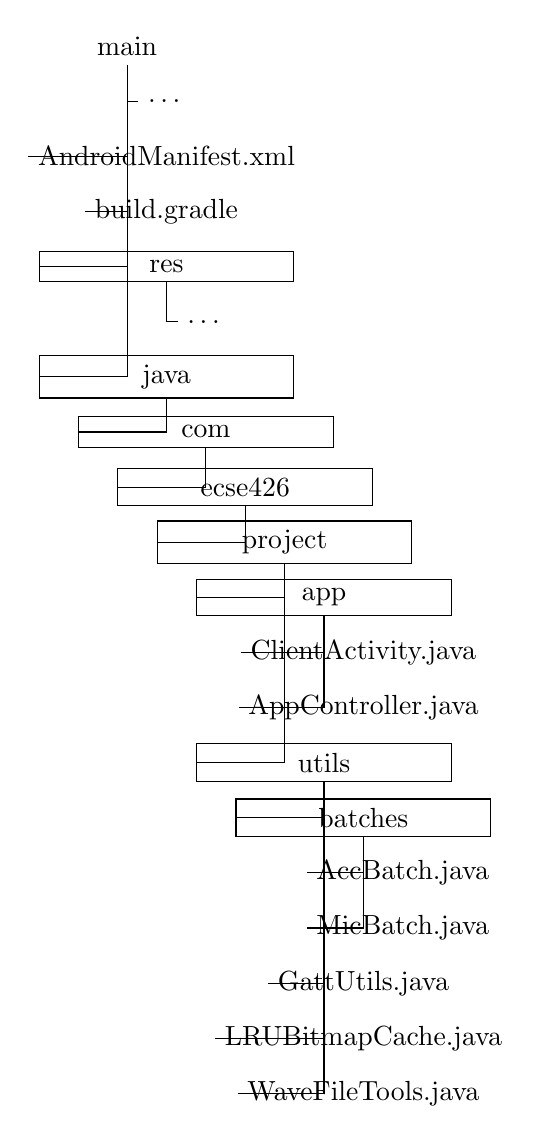
\begin{tikzpicture}[
	  grow via three points={one child at (0.5,-0.7) and
	  two children at (0.5,-0.7) and (0.5,-1.4)},   
	  edge from parent path={(\tikzparentnode.south) |- (\tikzchildnode.west)}]
	  \node {main}
		child { node [draw=none] {\ldots}}
		child { node [draw=none] {AndroidManifest.xml} }
		child { node [draw=none] {build.gradle} }
		child { node [label={[xshift=6.0cm, yshift=-0.58cm, color=gray]}] {res}
			child { node [draw=none] {\ldots}}
		}
		child [missing] {}
		child { node [label={[xshift=6.0cm, yshift=-0.58cm, color=gray]}] {java}
			child { node [label={[xshift=6.0cm, yshift=-0.58cm, color=gray]}] {com}
				child { node [label={[xshift=6.0cm, yshift=-0.58cm, color=gray]}] {ecse426}
					child { node [label={[xshift=6.0cm, yshift=-0.58cm, color=gray]}] {project}
						child { node [label={[xshift=6.0cm, yshift=-0.58cm, color=gray]}] {app}
							child { node [draw=none] {ClientActivity.java} }
							child { node [draw=none] {AppController.java} }
						}
						child [missing] {}
						child [missing] {}
						child { node [label={[xshift=6.0cm, yshift=-0.58cm, color=gray]}] {utils}
							child { node [label={[xshift=6.0cm, yshift=-0.58cm, color=gray]}] {batches}
							   child { node [draw=none] {AccBatch.java} } 
							   child { node [draw=none] {MicBatch.java} }
							}
							child [missing] {}
							child [missing] {}
							child { node [draw=none] {GattUtils.java} }
							child { node [draw=none] {LRUBitmapCache.java} }
							child { node [draw=none] {WaveFileTools.java} }
						}
					}
				}
			}
		};
	\end{tikzpicture}
\end{figure}
\tikzstyle{every node}=[] % resets borders of tables
\tikzstyle{selected}=[] % resets selected
The \texttt{AndroidManifest.xml} is the manifest file specific to this application which contains dependencies. The \texttt{build.gradle} file is the gradle build script, Android Studio automatically runs its build configurations whenever the developer runs or builds the application.\\

The \texttt{ClientActivity.java} class is the main activity that runs on start up. It is the core of the application, every other class is written around it and is used to help it. This class contains the BLE Scan Callback and GATT Client Callback logic implemented under inner classes. It handles user input and contains function calls from other classes that receive and save data over BLE and HTTP.\\

The \texttt{AppController.java} handles HTTP requests by facilitating the Client Activity with a queue for requests. It also handles reading and writing voice and accelerometer data to their appropriate files. It is important to note that the \texttt{AppController.java} class extends the Application class, making it able to run simultaneously with the \texttt{ClientActivity.java} class and have data persist when the application is closed.\\

The \texttt{AccBatch.java} and \texttt{MicBatch.java} classes are helper classes that contain functions to convert accelerometer or voice data respectively from bytes to a data type instructed by the function. The \texttt{GattUtils.java} class contains GATT Service, Characteristic, and Configuration UUIDs, as well as the Nucleo board's MAC address. The \texttt{WaveFileTools.java} class handles reading and writing data from and to files of Wave format. The \texttt{LRUBitmapCache.java} class is supposed to send and receive files, unfortunately it is not used.\\

Under the \texttt{res} directory, one can find all the user interface layouts and images. Any user interface design or image is found under that directory. 
